% This LaTeX was auto-generated from MATLAB code.
% To make changes, update the MATLAB code and export to LaTeX again.

\documentclass{article}
\usepackage[english, russian]{babel}
\usepackage[utf8]{inputenc}
\usepackage[T1]{fontenc}
\usepackage{lmodern}
\usepackage{graphicx}
\usepackage{color}
\usepackage{listings}
\usepackage{hyperref}
\usepackage{amsmath}
\usepackage{amsfonts}
\usepackage{epstopdf}
\usepackage{matlab}

\sloppy
\epstopdfsetup{outdir=./}
\graphicspath{ {./sound_ma_images/} }

\begin{document}

\begin{par}
\begin{flushleft}
1 Фильтрация сигнала методом скользящего среднего
\end{flushleft}
\end{par}

\begin{par}
\begin{flushleft}
1.1 Инициализация и формирование значений основных параметров
\end{flushleft}
\end{par}

\begin{matlabcode}
clear all; % Очистка памяти
close all; % Закрытие всех окон с графиками
clc; % Очистка окна команд и сообщений
fontSize = 10; % Размер шрифта графиков
tColor = 'b'; % Цвет графиков во временной области
fColor = [1 0.4 0]; % Цвет графиков в частотной области
A = 0.006; % Амплитуда шума
f0 = 5000; fn = 10000; df = 500; % Частота шума, Гц
w = 40; % Размер окна фильтра
\end{matlabcode}


\begin{par}
\begin{flushleft}
1.2 Чтение звукового файла
\end{flushleft}
\end{par}

\begin{matlabcode}
[data,rate] = audioread('sound.wav'); % Чтение отсчётов и частоты дискретизации
t = linspace(0, length(data)/rate, length(data)); % Формирование области определения
figure; plot(t, data, 'Color', tColor);
set(get(gcf, 'CurrentAxes'), 'FontSize', fontSize); % Изменение шрифта
title('\rm Исходный сигнал во временной области'); % Заголовок
xlabel('Время,\it nT_д\rm, с'); % Надпись оси абсцисс
ylabel('Сигнал,\it x(nT_д )\rm, В'); % Надпись оси ординат
\end{matlabcode}
\begin{center}
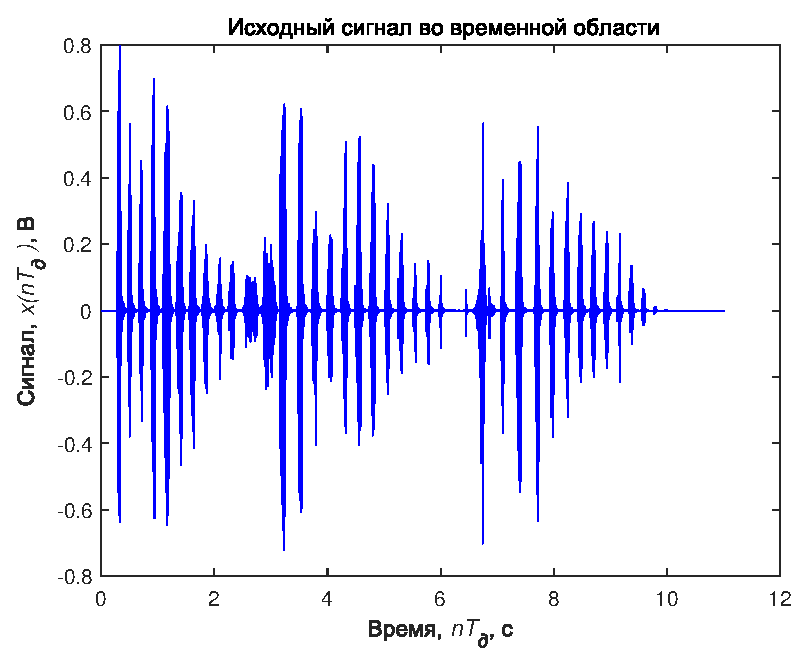
\includegraphics[width=\maxwidth{56.196688409433015em}]{figure_0}
\end{center}


\begin{par}
\begin{flushleft}
1.3 Построение амплитудного спектра исходного сигнала
\end{flushleft}
\end{par}

\begin{matlabcode}
f = linspace(0, rate, length(data)); % Формирование области определения
fdata = abs(fft(data)/length(data)); % Формирование значений спектра
figure; plot([-fliplr(f(1:end/2)) f(1:end/2)], fftshift(fdata),...
    'Color', fColor, 'LineWidth', 3);
axis([-rate/2 rate/2 0 A/2]); % Диапазон значений осей
set(get(gcf, 'CurrentAxes'), 'FontSize', fontSize); % Изменение шрифта
title('\rm Исходный сигнал в частотной области'); % Заголовок
xlabel('Частота,\it f\rm, Гц'); % Надпись оси абсцисс
ylabel('Амплитуда,\it A(f)\rm, В'); % Надпись оси ординат
\end{matlabcode}
\begin{center}
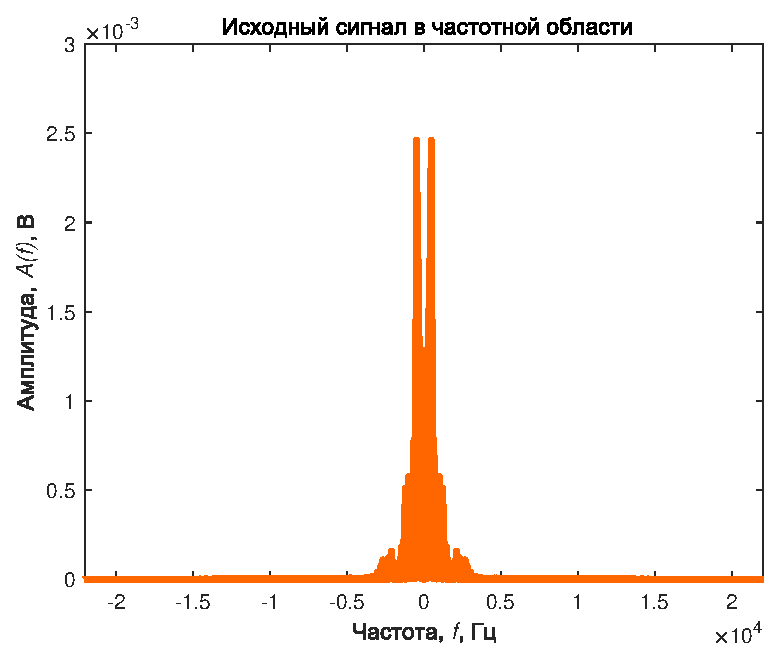
\includegraphics[width=\maxwidth{56.196688409433015em}]{figure_1}
\end{center}


\begin{par}
\begin{flushleft}
1.4 Формирование высокочастотного шума
\end{flushleft}
\end{par}

\begin{matlabcode}
ny=zeros(length(data),1); % Массив отсчётов шума
while f0 < fn
    ny=ny+A.*sin(2*pi*f0*t.');
    f0=f0+df;
end
fny = abs(fft(ny)/length(ny)); % Массив отсчётов спектра шума
figure; plot([-fliplr(f(1:end/2)) f(1:end/2)], fftshift(fny),...
    'Color', fColor, 'LineWidth', 3);
axis([-rate/2 rate/2 0 A/2]); % Диапазон значений осей
set(get(gcf, 'CurrentAxes'), 'FontSize', fontSize); % Изменение шрифта
title('\rm Высокочастотный шум в частотной области'); % Заголовок
xlabel('Частота,\it f\rm, Гц'); % Надпись оси абсцисс
ylabel('Амплитуда,\it A(f)\rm, В'); % Надпись оси ординат
\end{matlabcode}
\begin{center}
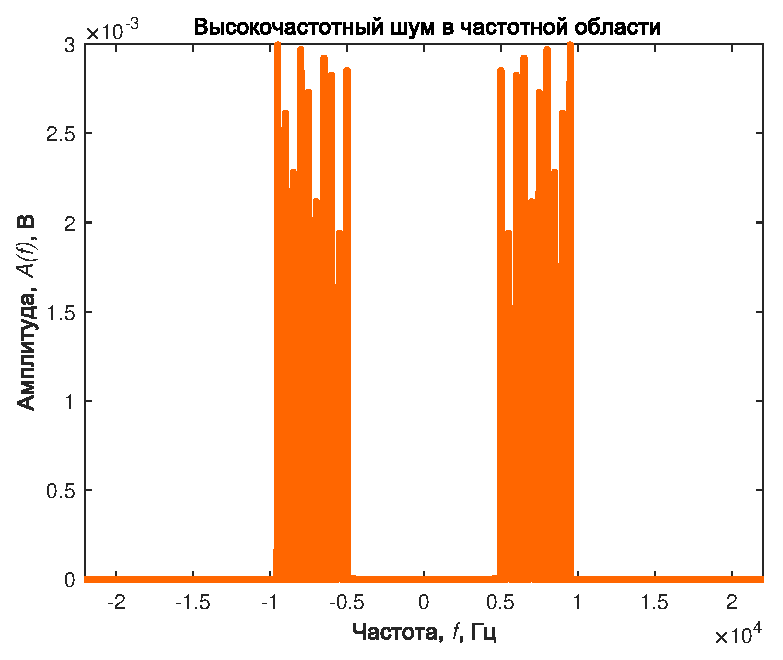
\includegraphics[width=\maxwidth{56.196688409433015em}]{figure_2}
\end{center}


\begin{par}
\begin{flushleft}
1.5 Формирование зашумлённого сигнала
\end{flushleft}
\end{par}

\begin{matlabcode}
ndata = data; % Массив отсчётов зашумлённого сигнала стереоканала
ndata(:,1) = data(:,1) + ny; % Добавление шума к исходному сигналу
ndata(:,2) = data(:,2) + ny;
% Запись звукового файла с зашумлённым сигналом
audiowrite('noise.wav', ndata, rate);
% Массив отсчётов спектра зашумлённого сигнала
fdata = abs(fft(ndata)/length(ndata));
figure; plot([-fliplr(f(1:end/2)) f(1:end/2)], fftshift(fdata),...
    'Color', fColor, 'LineWidth', 3);
axis([-rate/2 rate/2 0 A/2]); % Диапазон значений осей
set(get(gcf, 'CurrentAxes'), 'FontSize', fontSize); % Изменение шрифта
title('\rm Зашумлённый сигнал в частотной области'); % Заголовок
xlabel('Частота,\it f\rm, Гц'); % Надпись оси абсцисс
ylabel('Амплитуда,\it A(f)\rm, В'); % Надпись оси ординат
\end{matlabcode}
\begin{center}
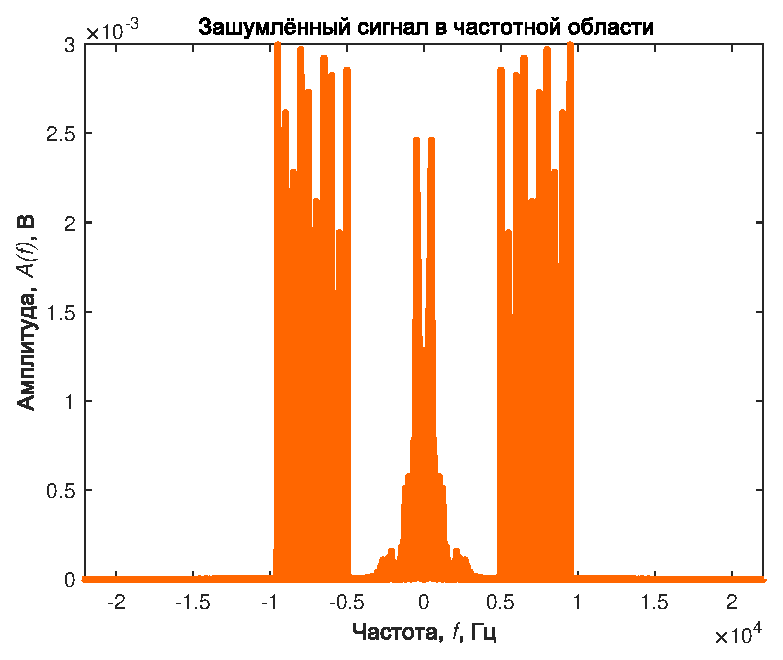
\includegraphics[width=\maxwidth{56.196688409433015em}]{figure_3}
\end{center}


\begin{par}
\begin{flushleft}
1.6 Фильтрация сигнала методом скользящего среднего
\end{flushleft}
\end{par}

\begin{matlabcode}
madata = ndata; % Массив отсчётов отфильтрованного сигнала стереоканала
% Фильтрация методом скользящего среднего с размером окна w
madata(:,1) = cumsum(ndata(:,1));
madata(:,2) = cumsum(ndata(:,2));
madata(w:end) = madata(w:end) - madata(1:end-w+1);
madata(w-1:end) = madata(w-1:end)./w;
% Запись звукового файла с отфильтрованным сигналом
audiowrite('filter.wav', madata, rate);
% Массив отсчётов спектра отфильтрованного сигнала
fdata = abs(fft(madata)/length(madata));
figure; plot([-fliplr(f(1:end/2)) f(1:end/2)], fftshift(fdata),...
    'Color', fColor, 'LineWidth', 3);
axis([-rate/2 rate/2 0 A/2]); % Диапазон значений осей
set(get(gcf, 'CurrentAxes'), 'FontSize', fontSize); % Изменение шрифта
title('\rm Отфильтрованный сигнал в частотной области'); % Заголовок
xlabel('Частота,\it f\rm, Гц'); % Надпись оси абсцисс
ylabel('Амплитуда,\it A(f)\rm, В'); % Надпись оси ординат
\end{matlabcode}
\begin{center}
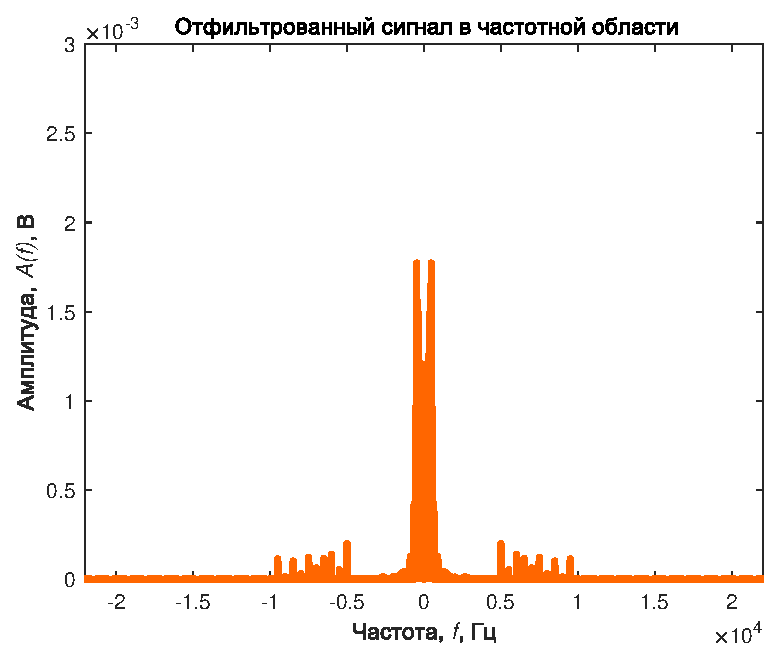
\includegraphics[width=\maxwidth{56.196688409433015em}]{figure_4}
\end{center}

\end{document}
